\documentclass[10pt]{beamer}

\mode<presentation>
{
	\usetheme{Frankfurt}
	\setbeamercovered{transparent}
}

\usepackage[spanish]{babel}
\usepackage[latin1]{inputenc}
\usepackage{subfigure}
\usepackage{bm}
\usepackage{booktabs}

\title[Aprendizaje Autom\'atico]{Algoritmos de Aprendizaje Autom\'atico y sus aplicaciones}
\subtitle{Trabajo de Fin de Grado}
\author{Javier D\'iaz Bustamante Ussia}
\institute{Universidad Complutense de Madrid}
\date[16/09/15]{16 de septiembre de 2015}

\graphicspath{{./graficas/}}

\begin{document}

\begin{frame}
	\titlepage
\end{frame}

\section{Motivaci\'on}

\begin{frame}
	\frametitle{Aplicaciones del Machine Learning}
	\begin{itemize}
		\item Motores de b\'usqueda
		\item Reconocimiento de escritura y voz
		\item Reconocimiento facial
		\item Sistemas de recomendaciones
		\item Detecci\'on de mensajes SPAM
		\item Detecci\'on de fraudes en transacciones con tarjetas de cr\'edito
		\item Conducci\'on aut\'onoma
		\item Clasificaci\'on de secuencias de ADN
		\item B\'usqueda del bos\'on de Higgs
		\item ...
	\end{itemize}
\end{frame}

\begin{frame}
	\frametitle{?`C\'omo ayuda a buscar el Higgs?}
	\centering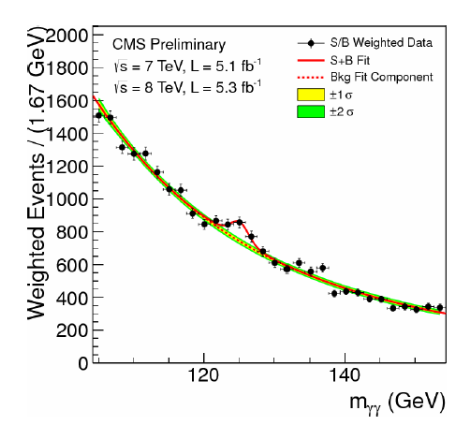
\includegraphics[width = 0.7\textwidth]{exceso_eventos_higgs}
\end{frame}

\section{Conceptos b\'asicos}

\subsection{Clasificaci\'on vs. Regresi\'on}

\begin{frame}
	\frametitle{Clasificaci\'on vs. Regresi\'on}
		\begin{figure}[htbp]
		\centering
		\subfigure{\includegraphics[width=0.4\textwidth]{NoBiasVariance}}
		\qquad\quad
		\subfigure{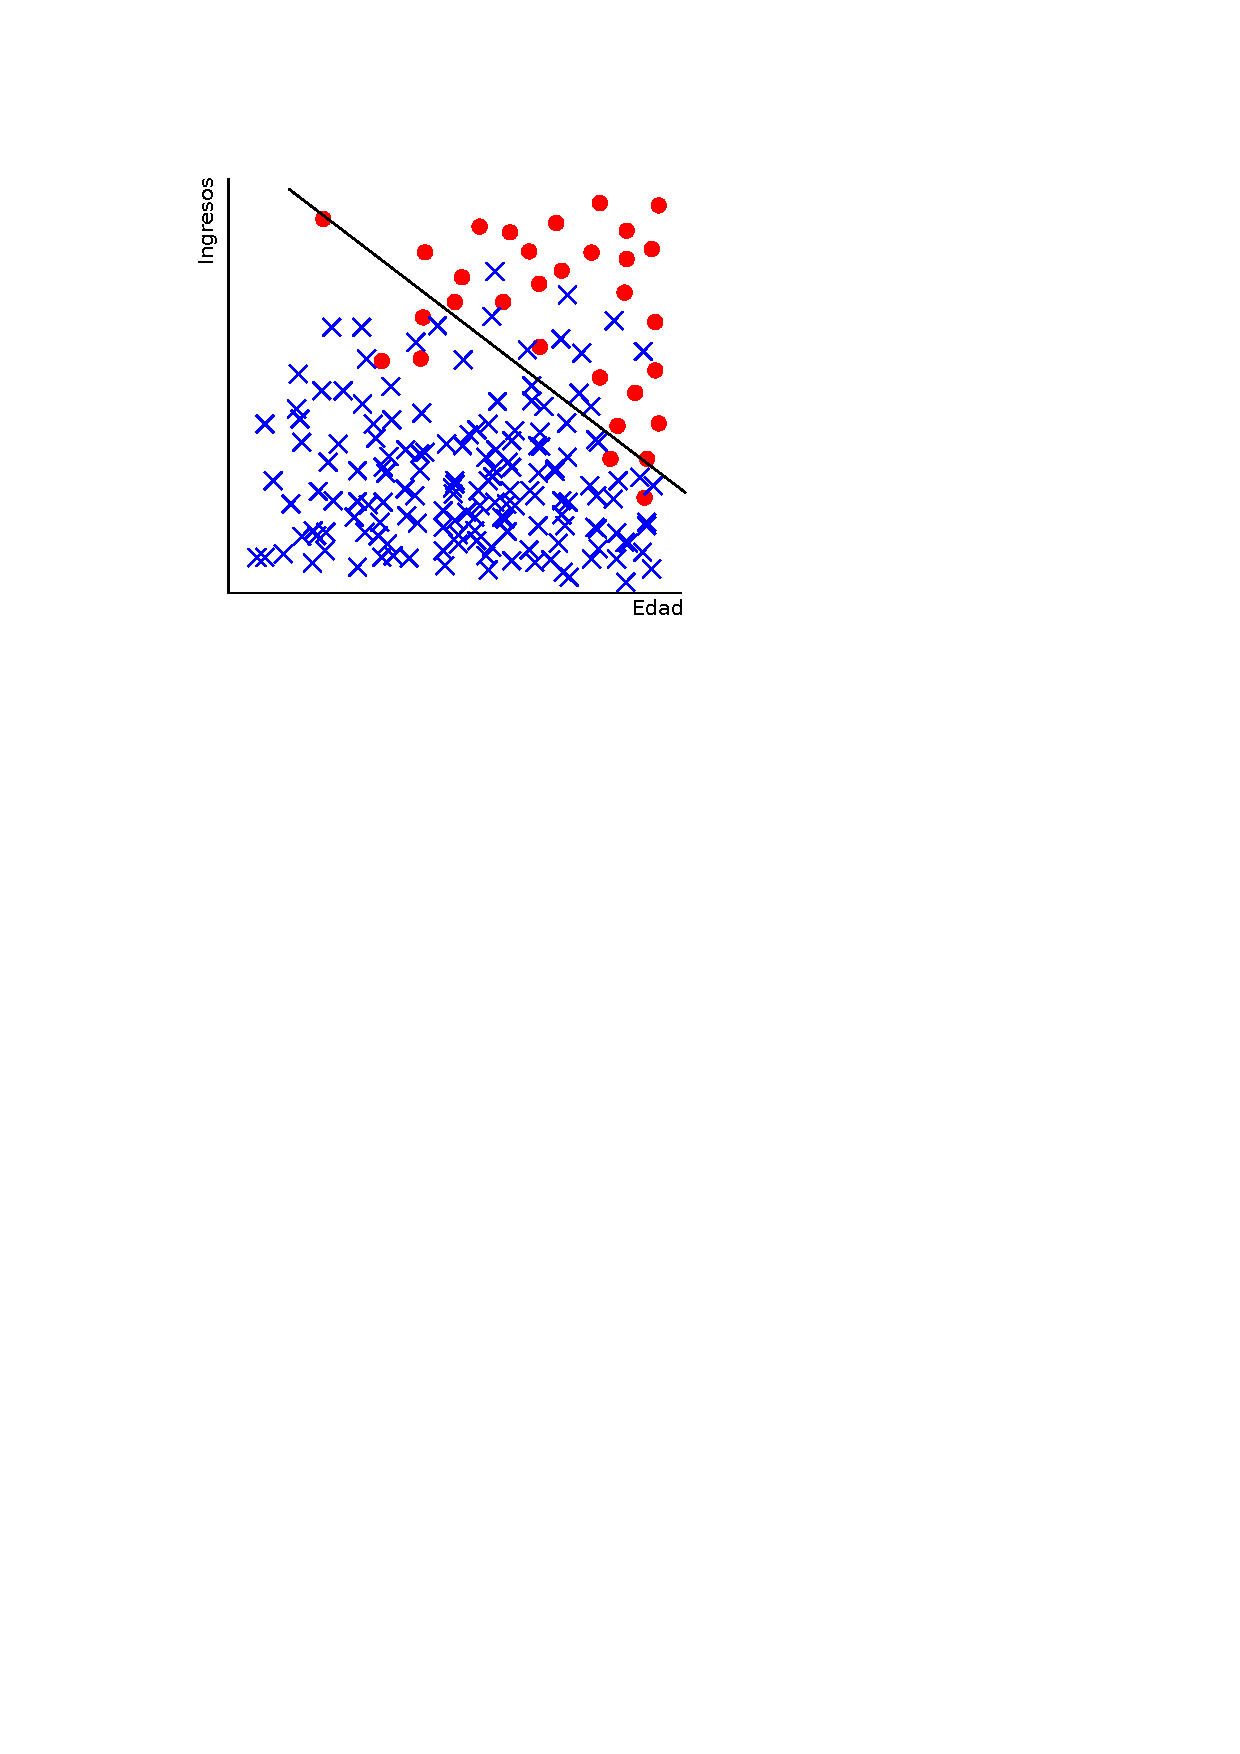
\includegraphics[width=0.4\textwidth]{supervisadoDecCurv}}
	\end{figure}
	
\end{frame}

\subsection{Supervisado o no supervisado}

\begin{frame}
	\frametitle{Supervisado o no supervisado}
	\begin{figure}[htbp]
	\centering
	\subfigure{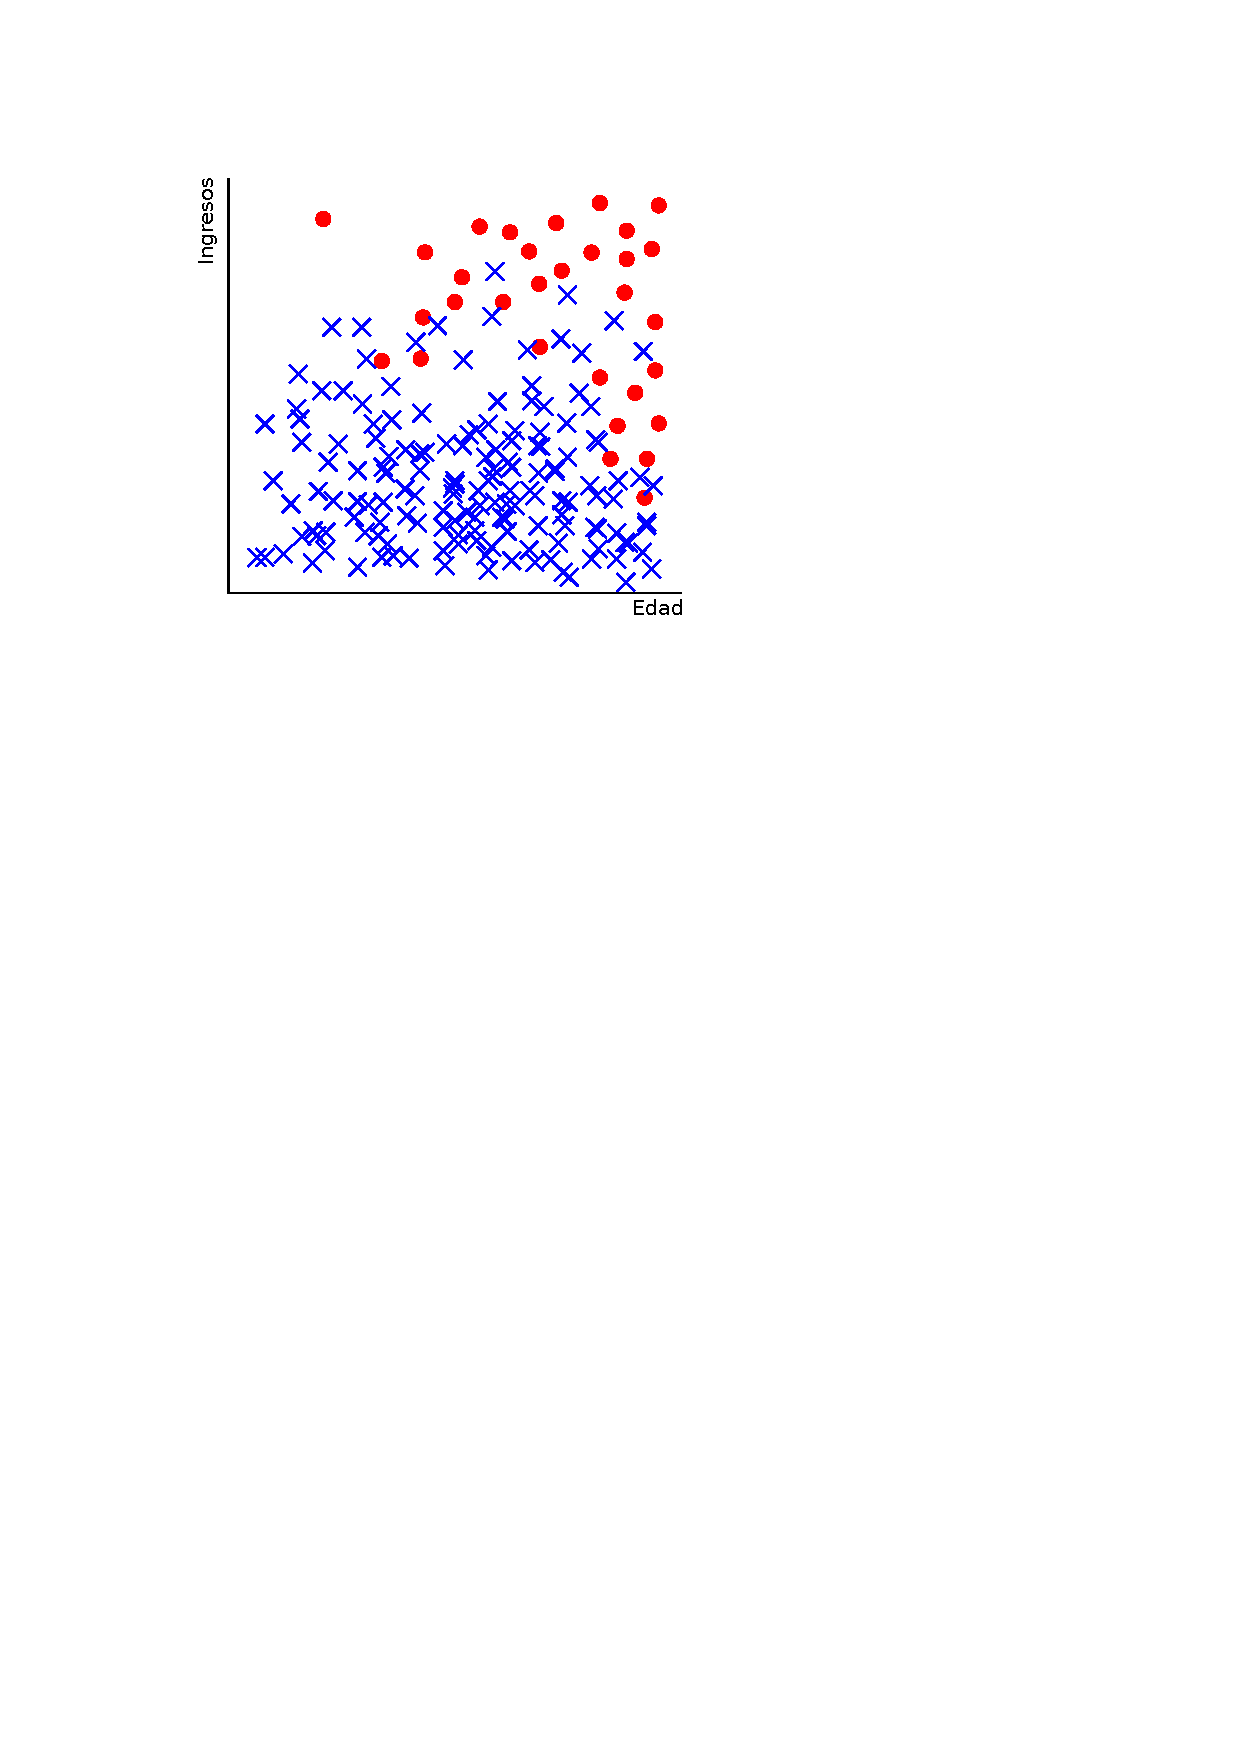
\includegraphics[width=0.4\textwidth]{supervisado}}
	\qquad\quad
	\subfigure{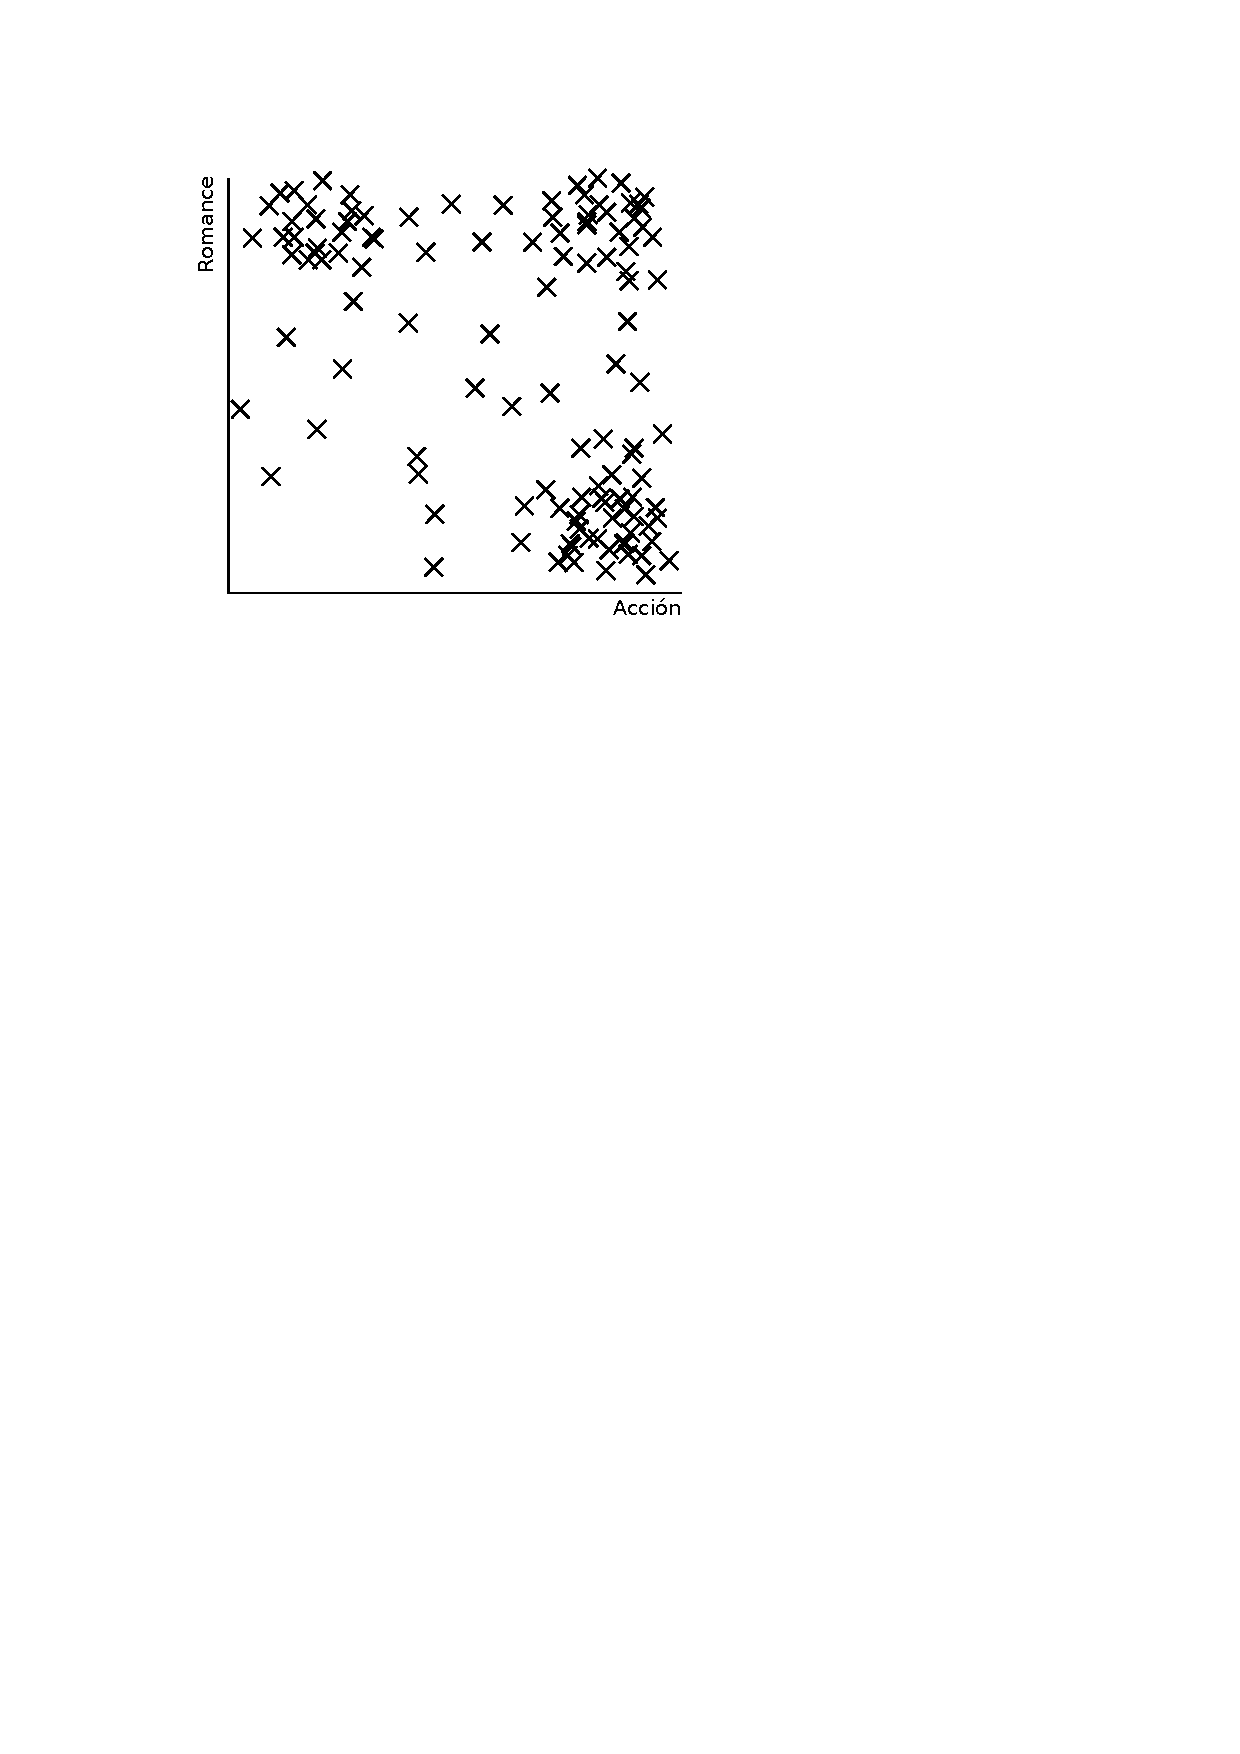
\includegraphics[width=0.4\textwidth]{noSupervisado}}
\end{figure}
\end{frame}

\subsection{Superficies de decisi\'on}

\begin{frame}
	\frametitle{Superficies de decisi\'on}
	\centering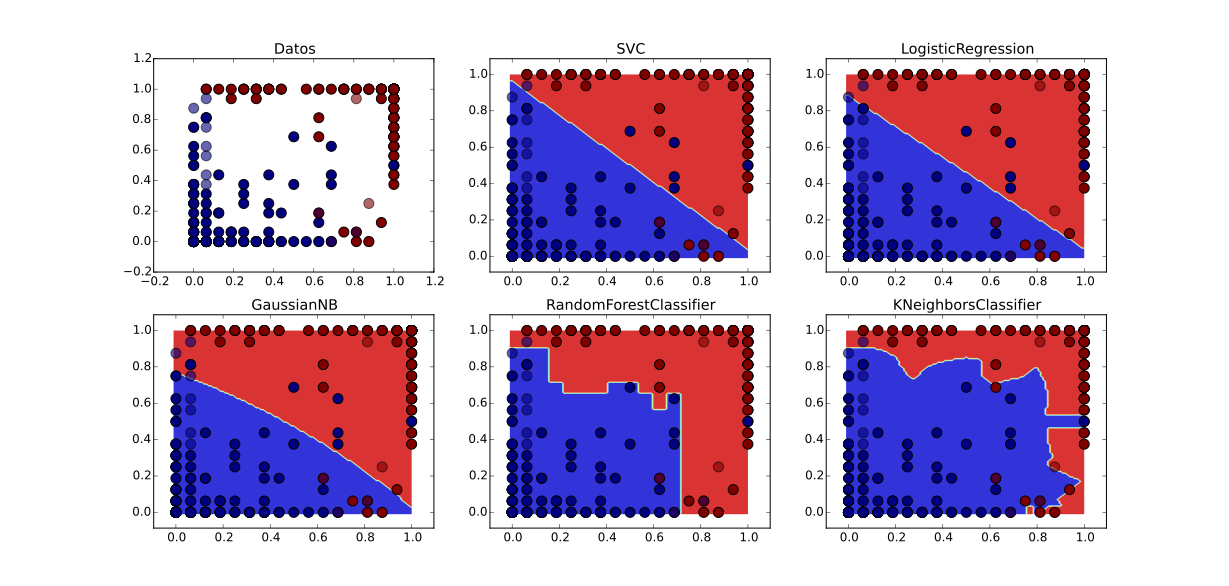
\includegraphics[width = 1.0\textwidth]{digitos,_curvas_de_decision21-28}
\end{frame}

\subsection{Sesgo y varianza}

\begin{frame}
	\frametitle{Sesgo y varianza}
		\begin{figure}[htbp]
		\centering
		\subfigure{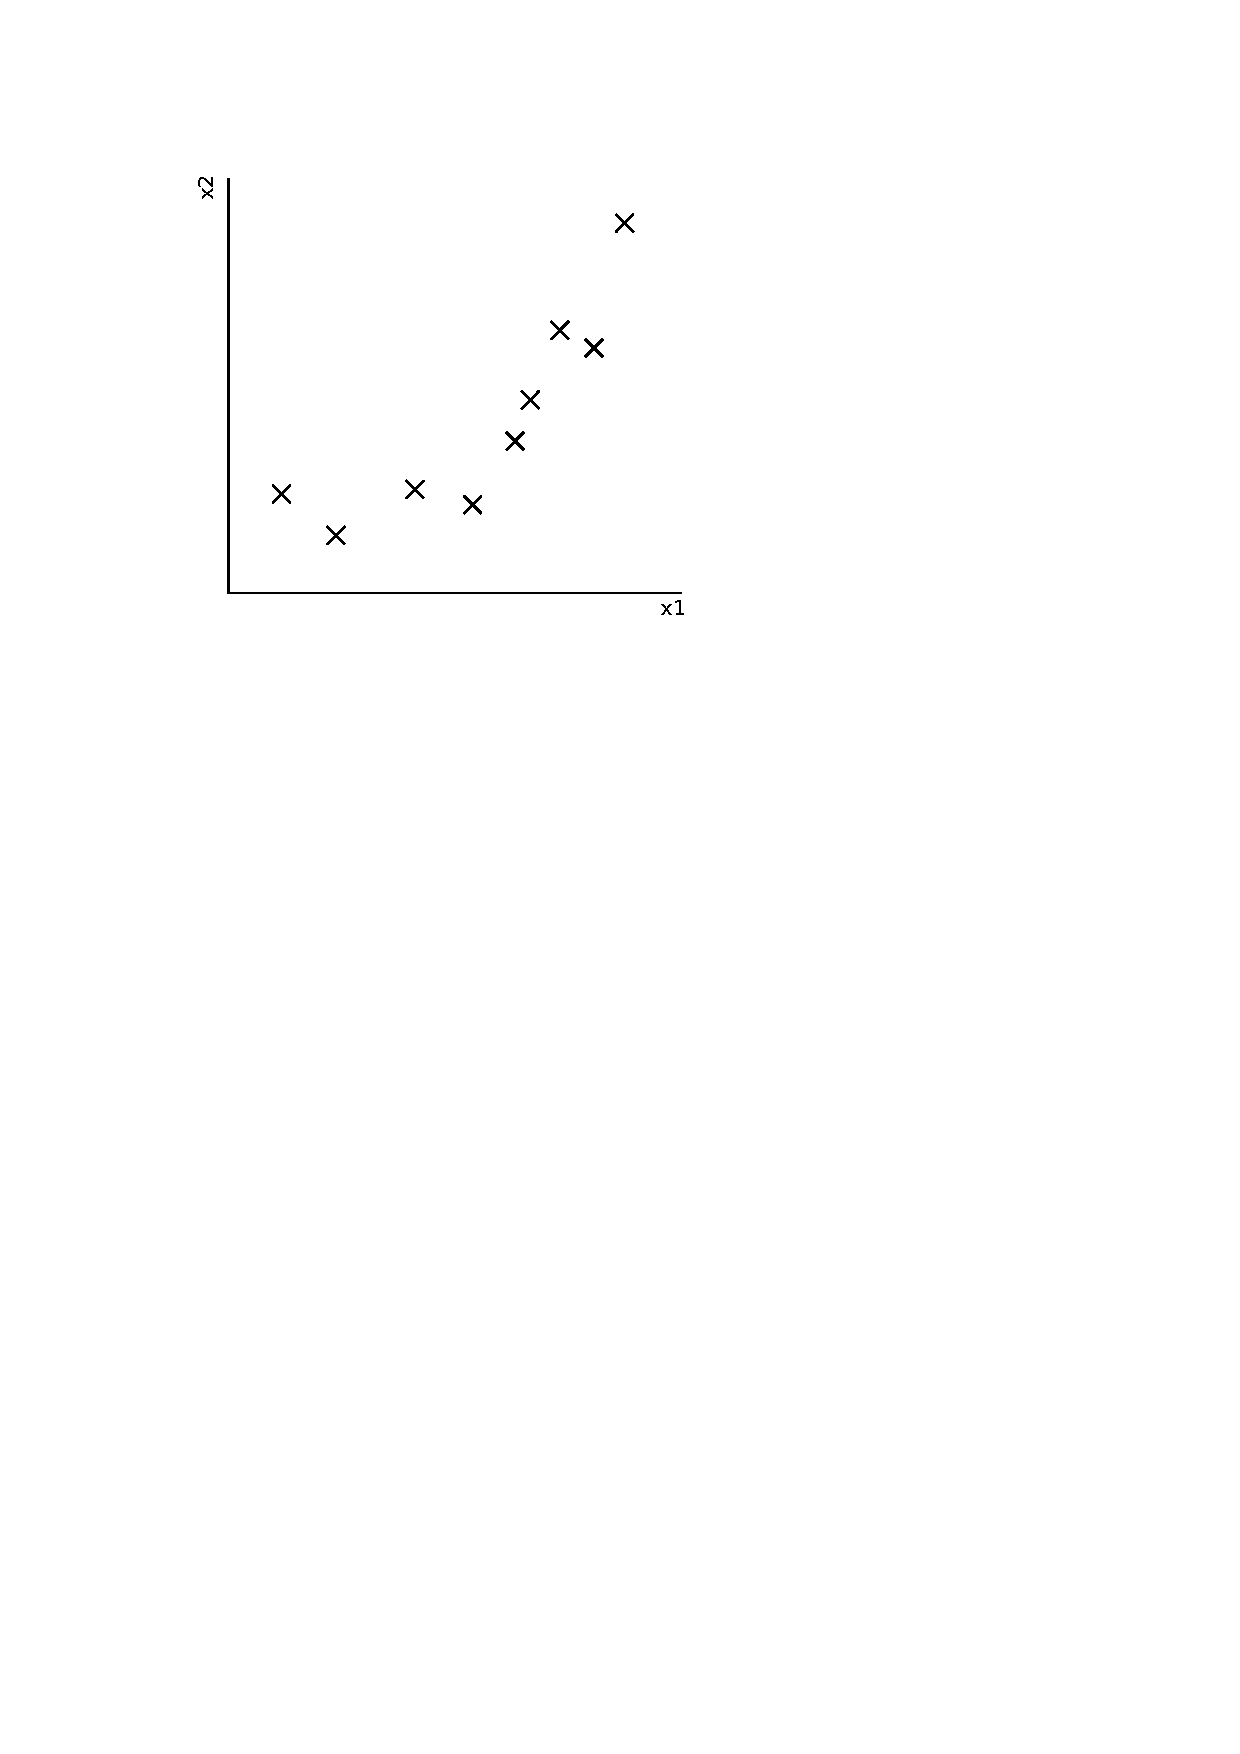
\includegraphics[width=0.35\textwidth]{DatosBiasVariance}}
		\qquad\quad
		\subfigure{\includegraphics[width=0.35\textwidth]{NoBiasVariance}}
		\qquad\quad
		\subfigure{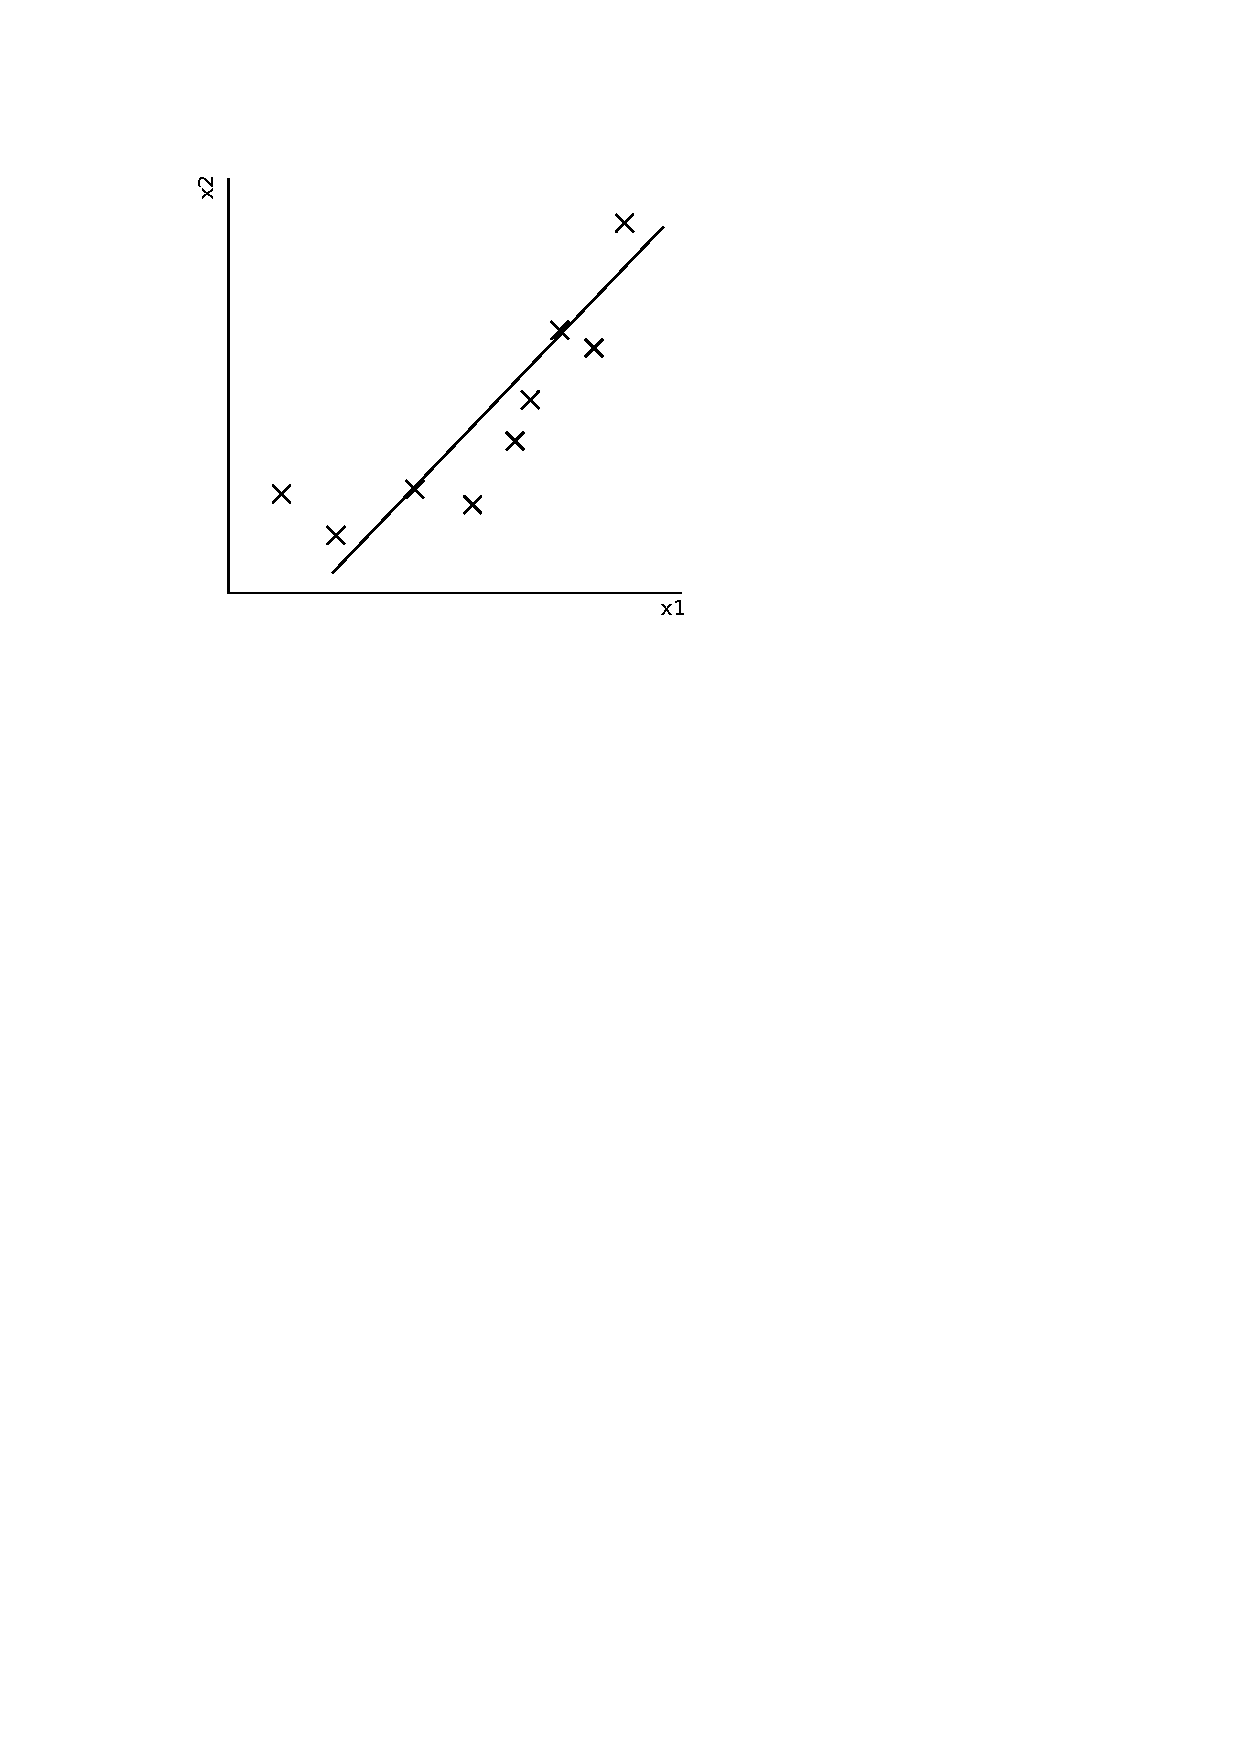
\includegraphics[width=0.35\textwidth]{highBias}}
		\qquad\quad
		\subfigure{\includegraphics[width=0.35\textwidth]{highVariance}}
	\end{figure}
\end{frame}

\subsection{M\'etricas}

\begin{frame}
	\frametitle{M\'etricas}
	\begin{table}[htbp]
		\centering
		\begin{tabular}{|c|c|c|}
			\hline
			& \textbf{0 real} & \textbf{1 real} \\
			\hline
			\textbf{0 predicho} & Verdadero negativo (TN) & Falso negativo (FN) \\
			\hline
			\textbf{1 predicho} & Falso positivo (FP) & Verdadero positivo (TP) \\
			\hline
		\end{tabular}
	\end{table}

	\begin{equation*}
		\begin{aligned}
			\text{Accuracy} &= \frac{TP + TN}{TP + FP + TN + FN} & \text{Recall} &= \frac{TP}{TP + FN} \\
			\text{Specificity} &= \frac{TN}{FP + TN} & \text{Precision} &= \frac{TP}{TP + FP} \\
			\text{F1-score} &= \frac{2\cdot \text{Precision}\cdot \text{Recall}}{\text{Precision} + \text{Recall}} & &
		\end{aligned}
	\end{equation*}
\end{frame}

\section{Algoritmos}

\subsection{K-Nearest Neighbors}

\begin{frame}
	\frametitle{K-Nearest Neigbors}
	\begin{figure}[htbp]
		\centering
		\subfigure{\includegraphics[width=0.35\textwidth]{KNN}}
		\qquad\quad
		\subfigure{\includegraphics[width=0.35\textwidth]{KNN1}}
		\subfigure{\includegraphics[width=0.35\textwidth]{KNN1Overfit}}
		\qquad\quad
		\subfigure{\includegraphics[width=0.35\textwidth]{KNN3}}
	\end{figure}
\end{frame}

\subsection{Logistic Regression}

\begin{frame}
	\frametitle{Logistic Regression}
	\begin{figure}[htbp]
		\centering
		\subfigure{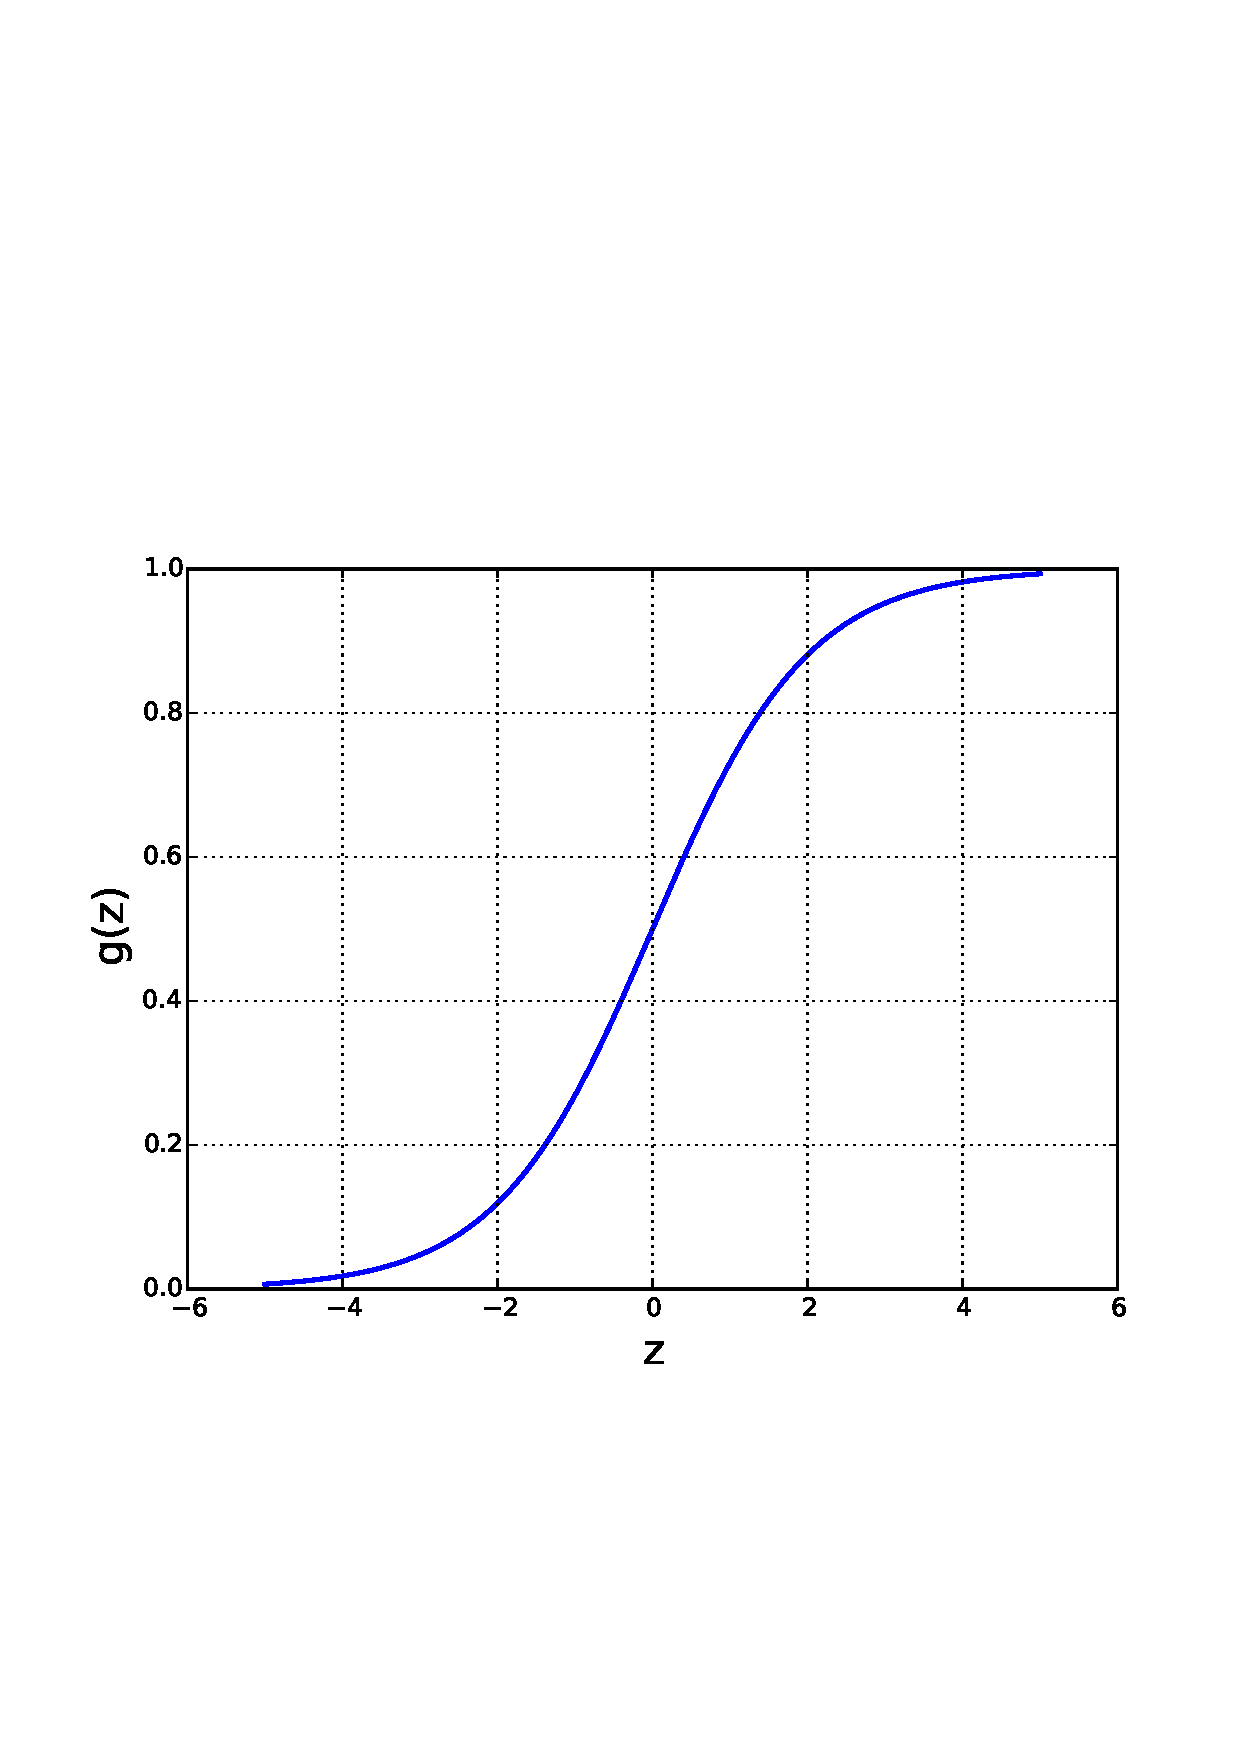
\includegraphics[width=0.45\textwidth]{sigmoid}}
		\subfigure{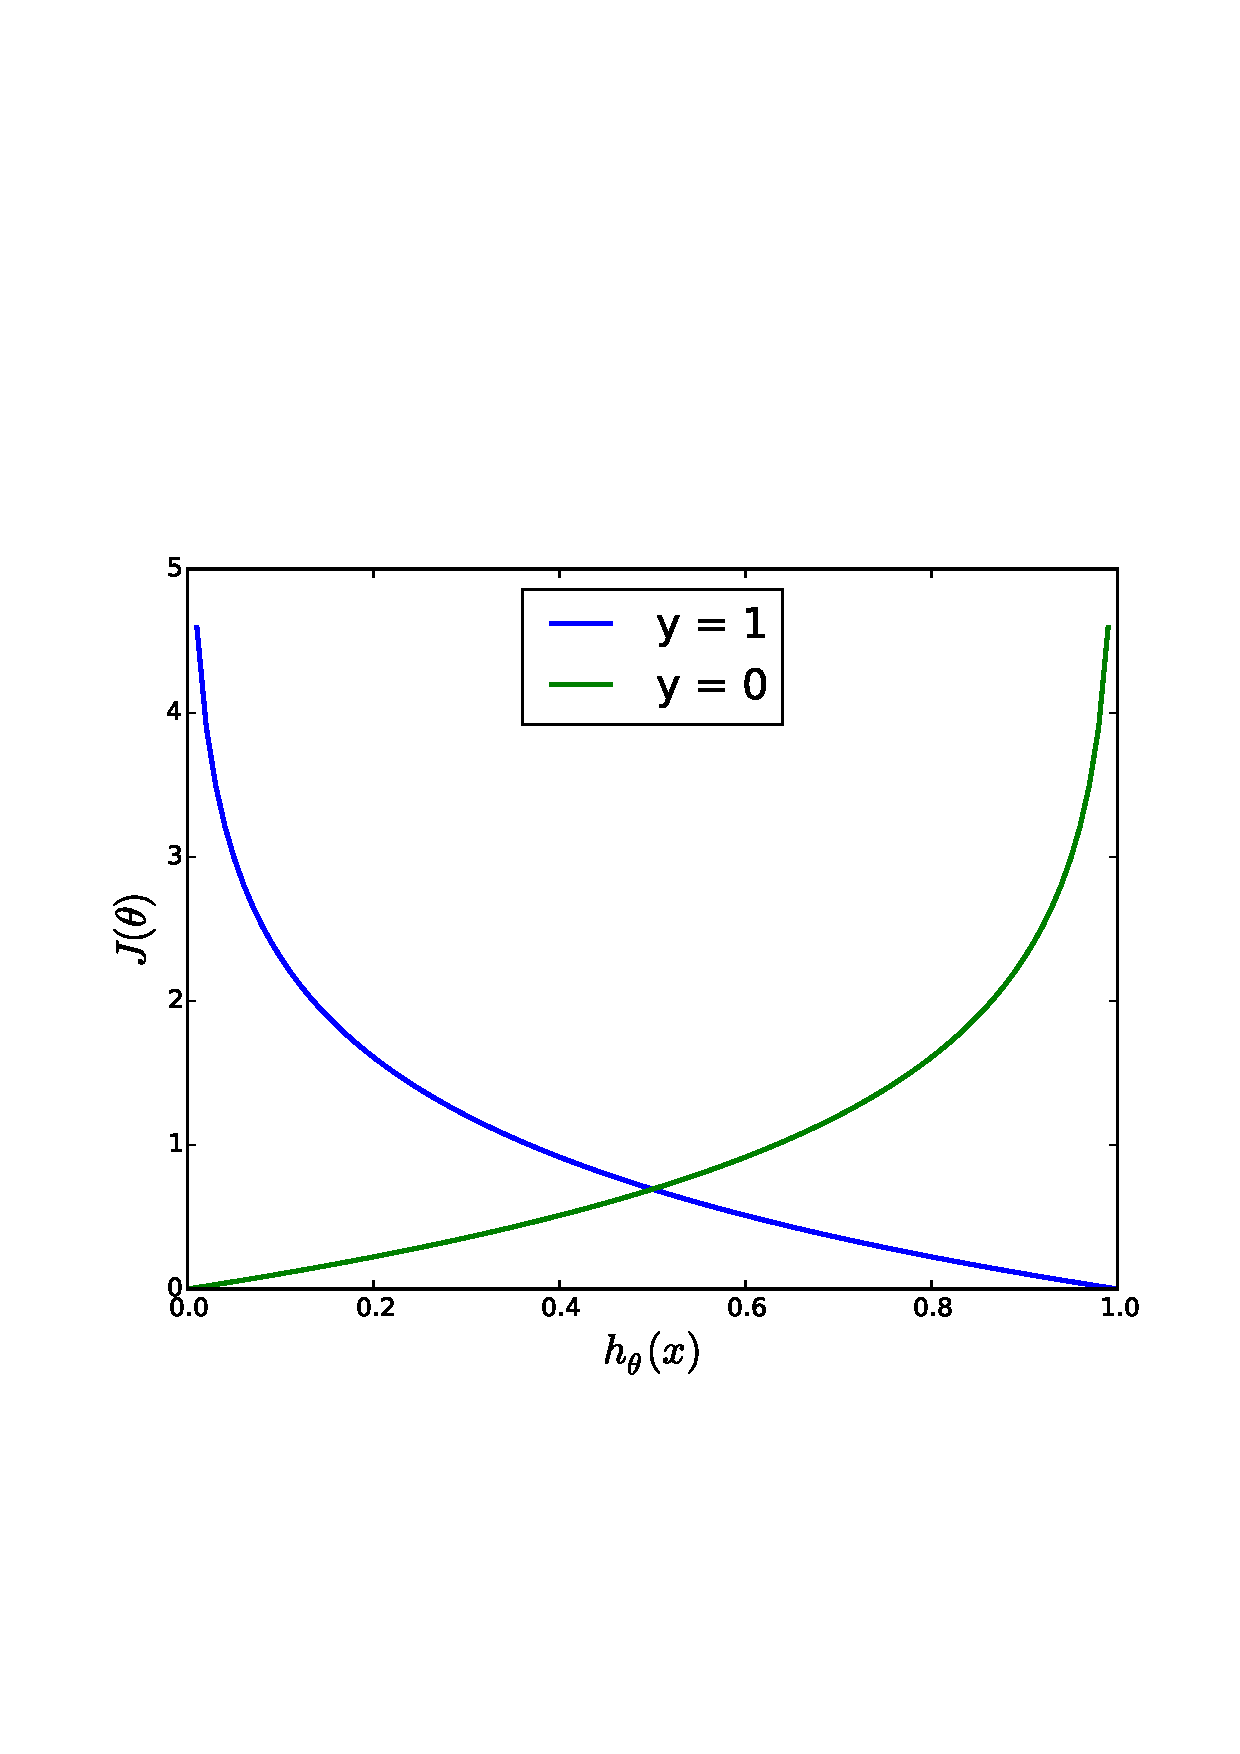
\includegraphics[width=0.45\textwidth]{costLogReg}}
	\end{figure}
\end{frame}

\subsection{Na\"ive Bayes}

\begin{frame}
	\frametitle{Na\"ive Bayes}
	\[p(C_l|\bm{x}) = \frac{p(C_l)p(\bm{x}|C_l)}{p(\bm{x})}\]
	
	\[p(\bm{x}|C) = \prod_{j=1}^n{p(x_j|C)}\]
	
	\[k = \underset{l}{\operatorname{max}}\ p(C_l|\bm{x})\]
\end{frame}

\subsection{Support Vector Machines}

\begin{frame}
	\frametitle{Support Vector Machines}
	\centering\includegraphics[width=0.7\textwidth]{highMargin}
\end{frame}

\begin{frame}
	\frametitle{Support Vector Machines}
	\begin{figure}[htbp]
		\centering
		\subfigure{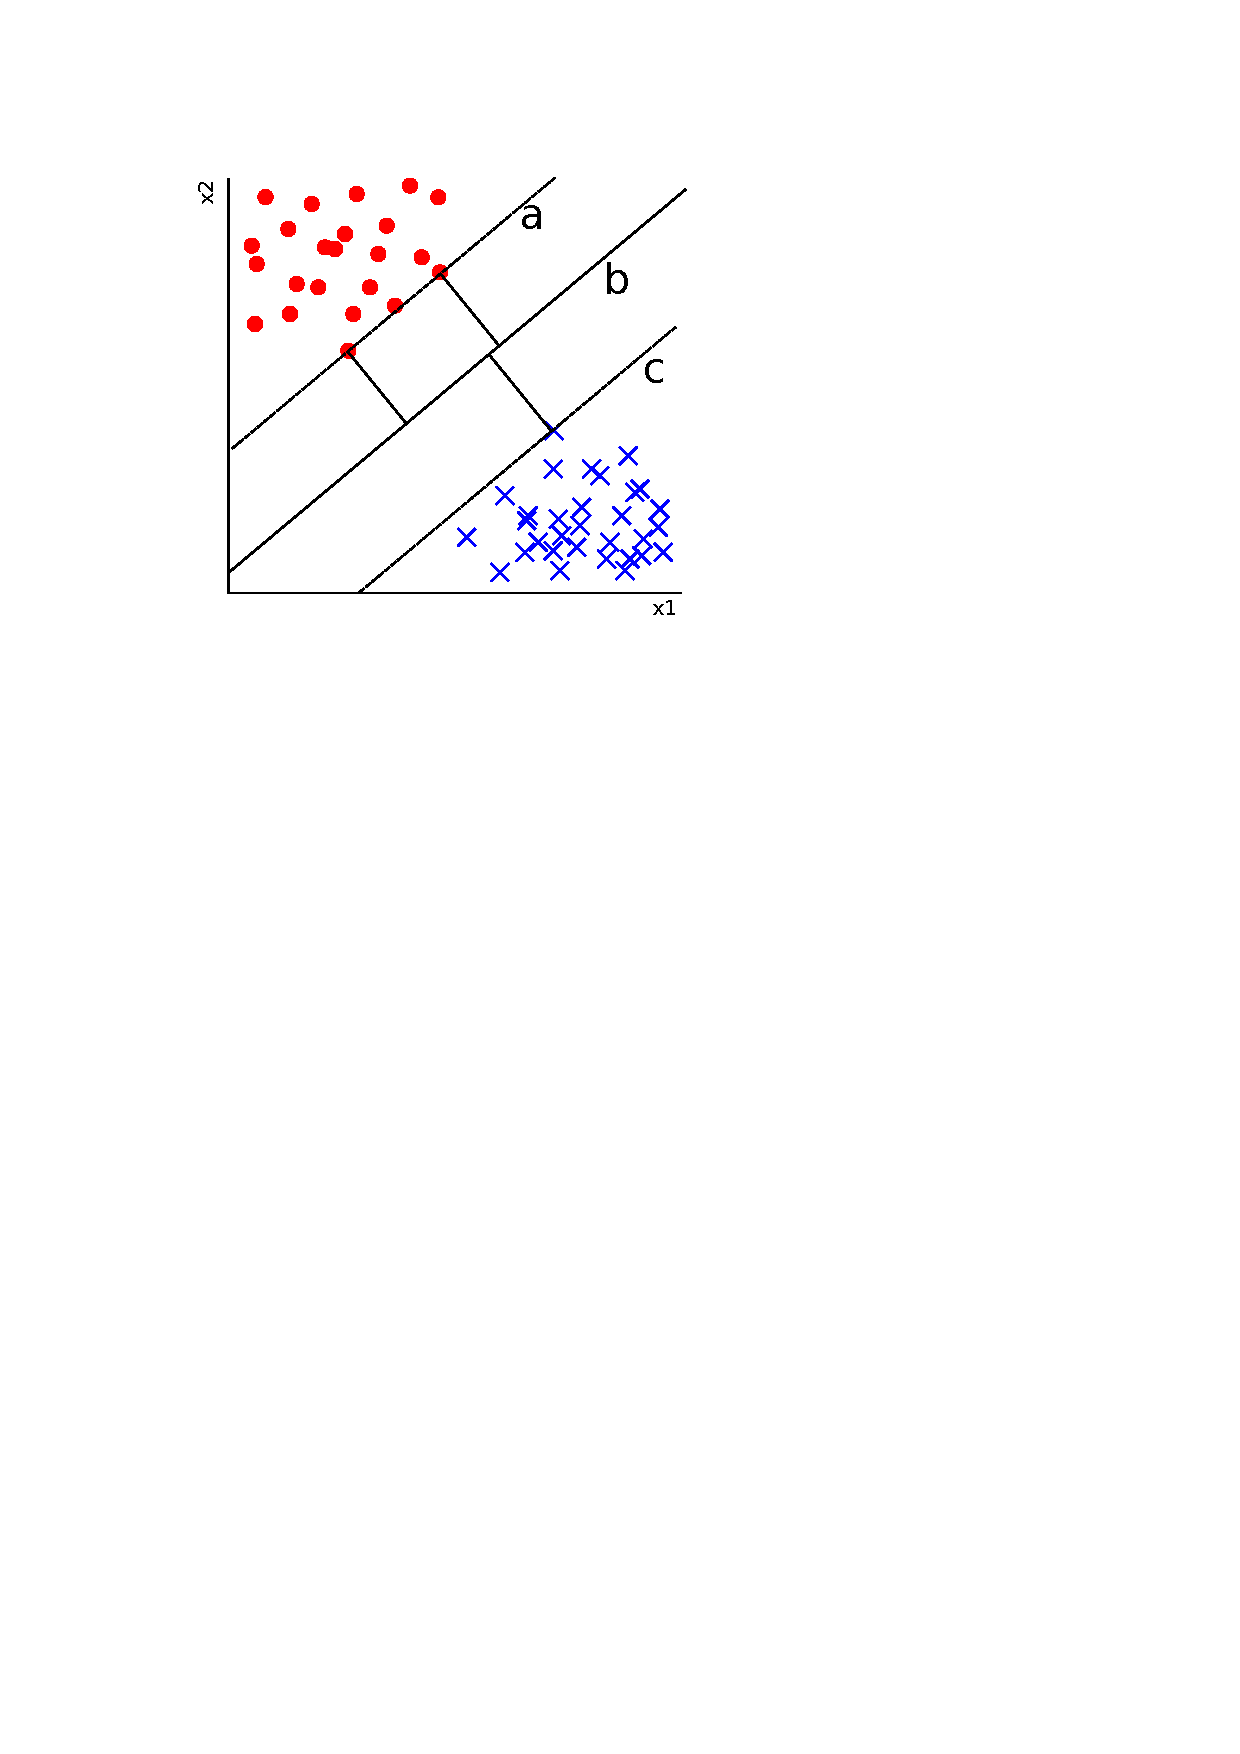
\includegraphics[width=0.4\textwidth]{highMargin2}}
		\qquad\quad
		\subfigure{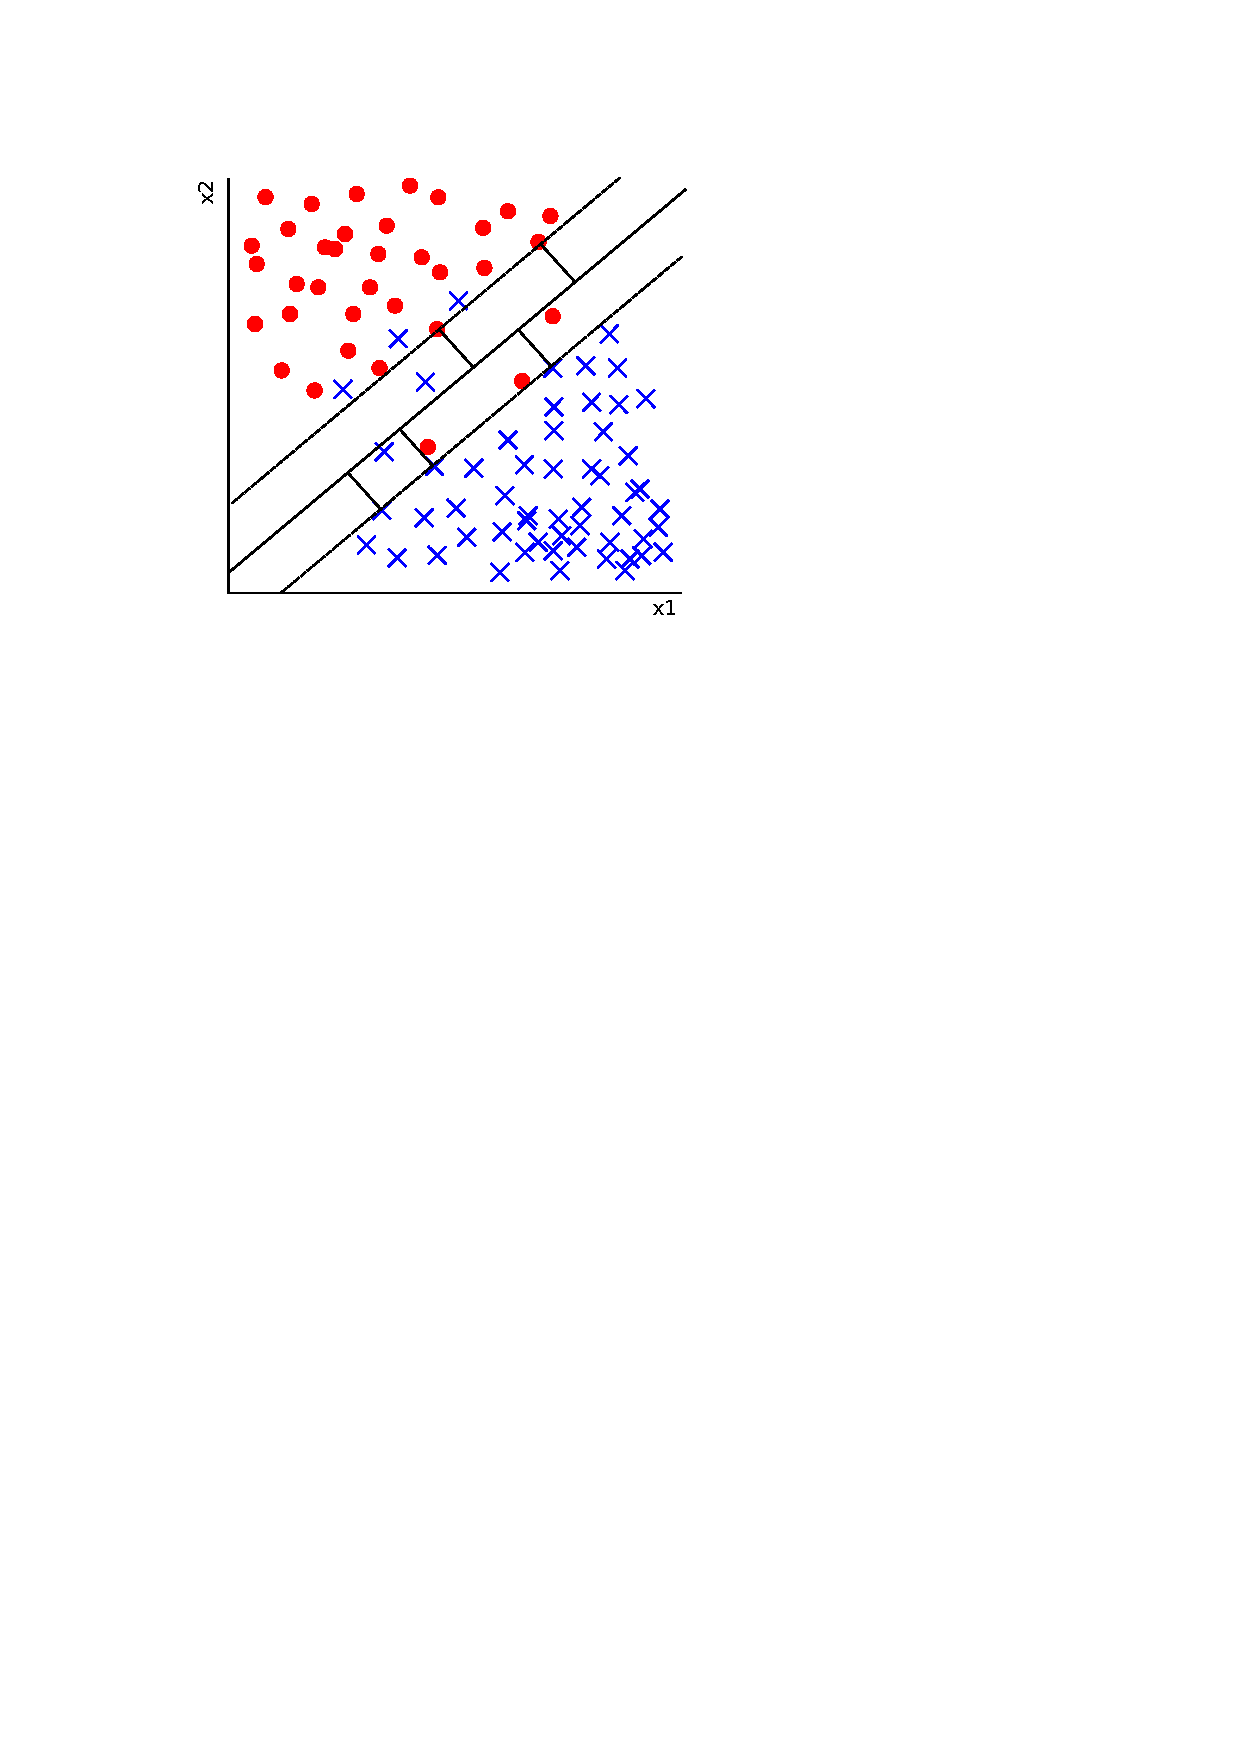
\includegraphics[width=0.4\textwidth]{softMargin}}
	\end{figure}
\end{frame}

\subsection{Random Forest}

\begin{frame}
	\frametitle{Random Forest, \'arboles de decisi\'on}
	\begin{figure}[htbp]
		\centering
		\subfigure{\includegraphics[width=0.4\textwidth]{RandomForest}}
		\qquad\quad
		\subfigure{\includegraphics[width=0.4\textwidth]{DecTreeOverfit}}
	\end{figure}
\end{frame}

\begin{frame}
	\frametitle{Random Forest, ensemble methods}
	\centering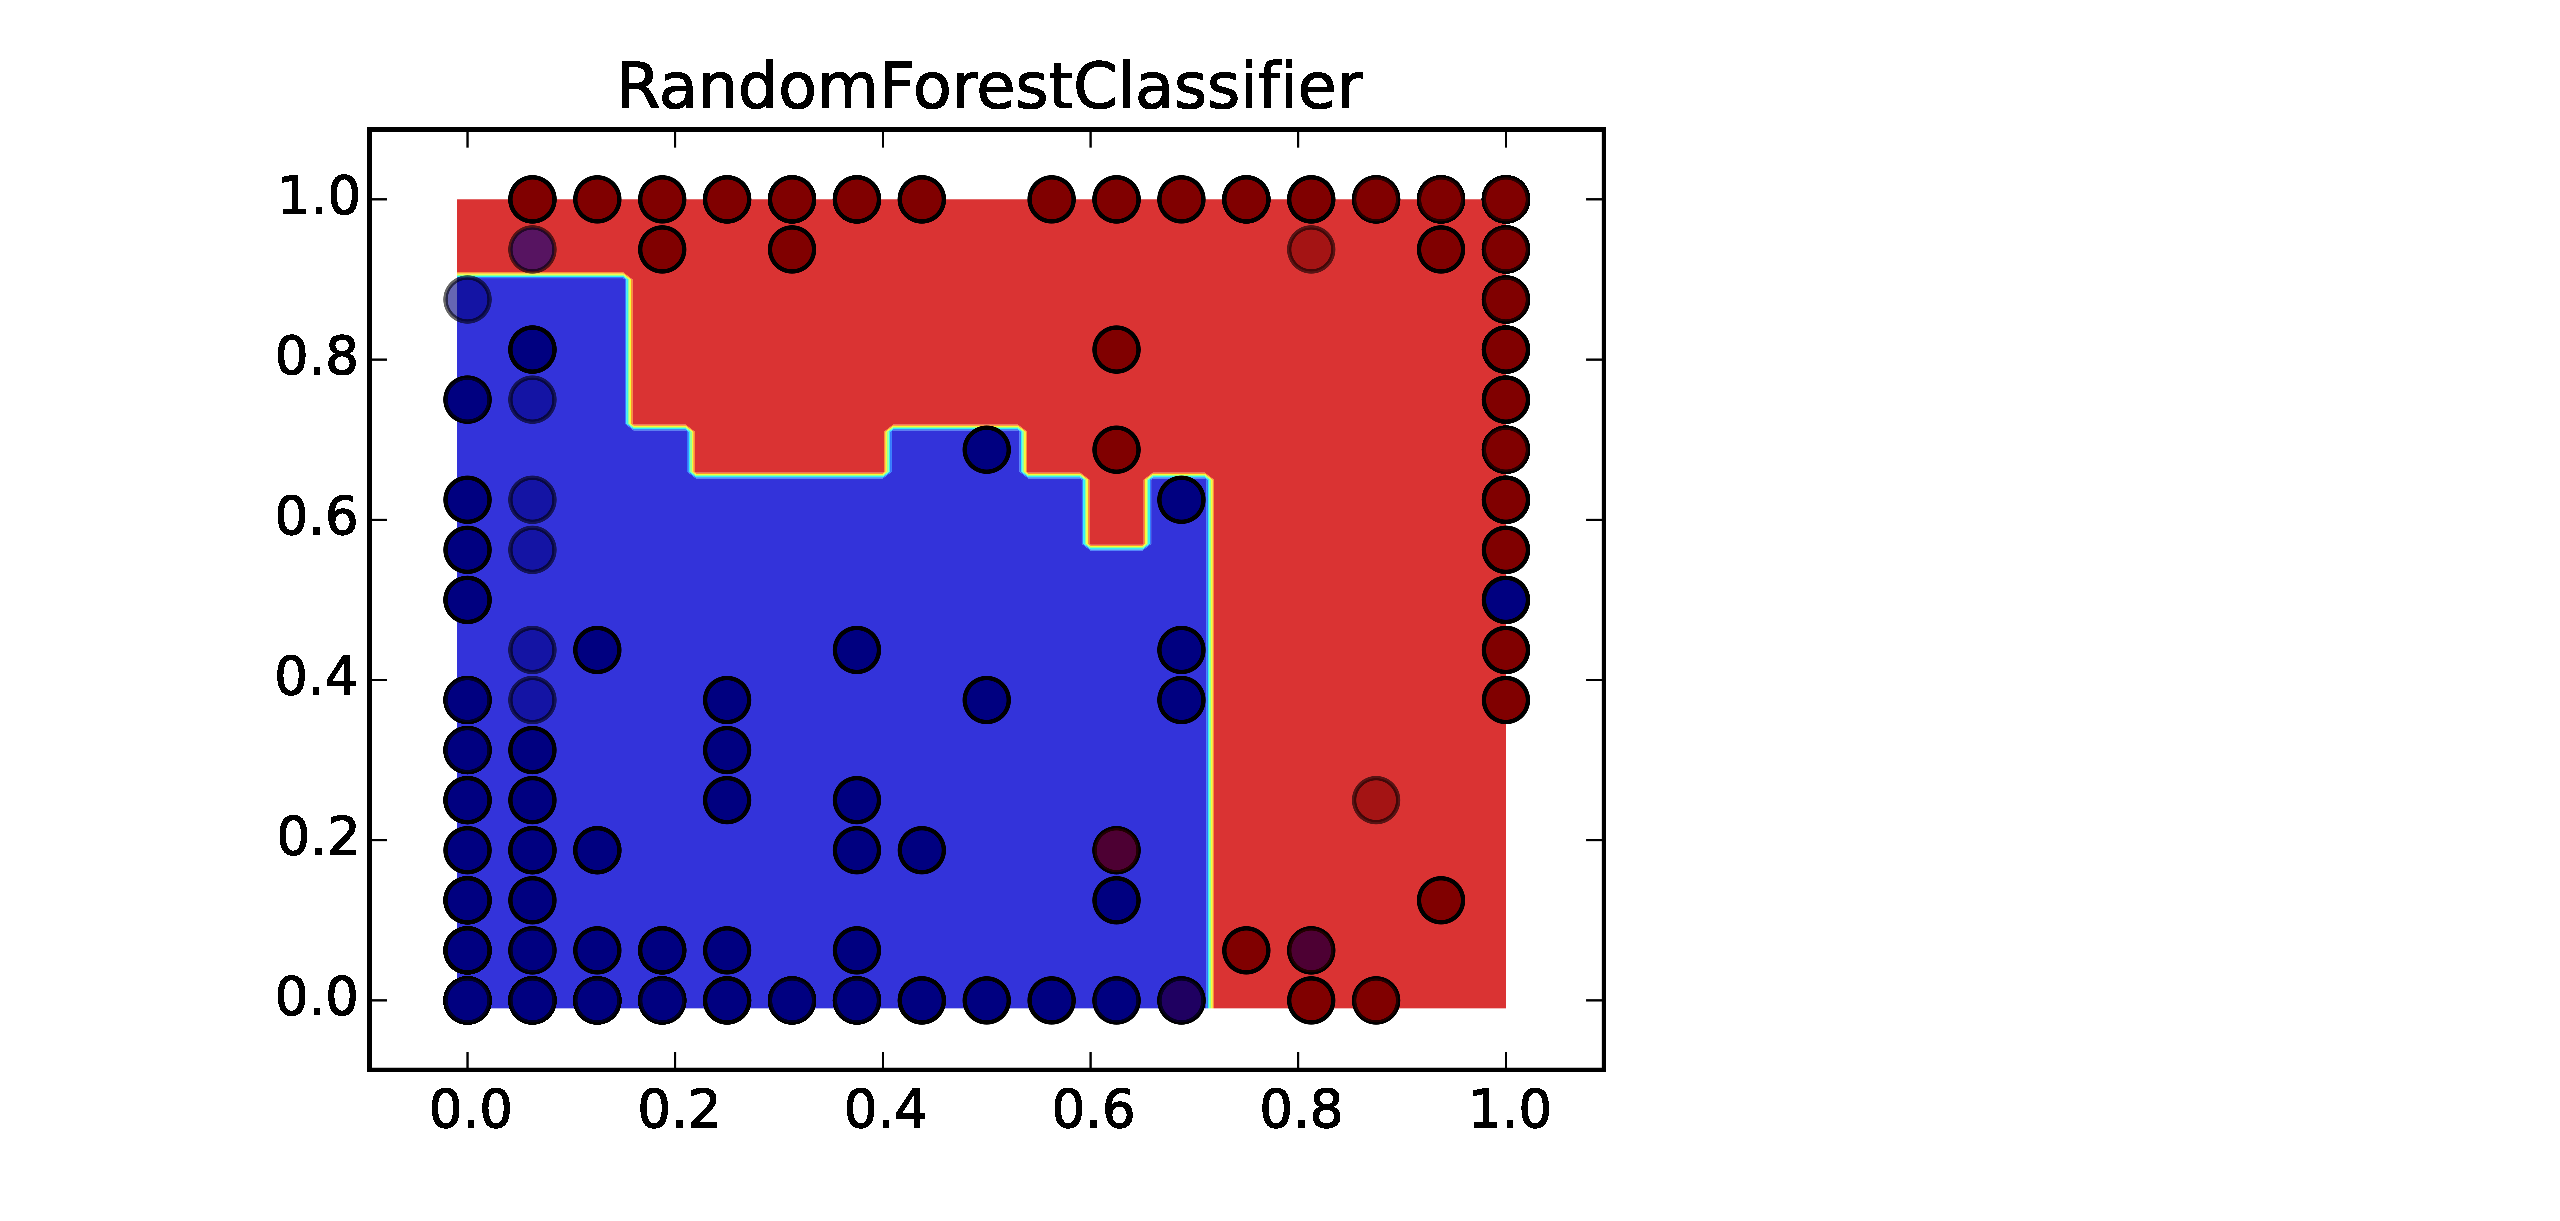
\includegraphics[width=0.7\textwidth]{curva_decision_RF}
\end{frame}

\section{Resultados}

\begin{frame}
	\frametitle{Resultados, el Higgs}
	\begin{table}[htbp]
		\centering
		\begin{tabular}{ccccc}
		  \toprule
			Algoritmo & Accuracy & Precision & Recall & F1-Score \\
			\midrule
			Gaussian NB & 0.6858 & 0.7367 & 0.8144 & 0.7736 \\
			SVM & 0.8129 & 0.8413 & 0.8826 & 0.8614 \\
			Logistic Regression & 0.7412 & 0.7810 & 0.8608 & 0.8190 \\
			Random Forest & 0.8252 & 0.8450 & 0.9000 & 0.8716 \\
			KNN & 0.7249 & 0.7855 & 0.8015 & 0.7934 \\
			\bottomrule
			\end{tabular}
\end{table}
\end{frame}

\begin{frame}
	\frametitle{Resultados, el Higgs}
	\begin{figure}[htbp]
		\centering
		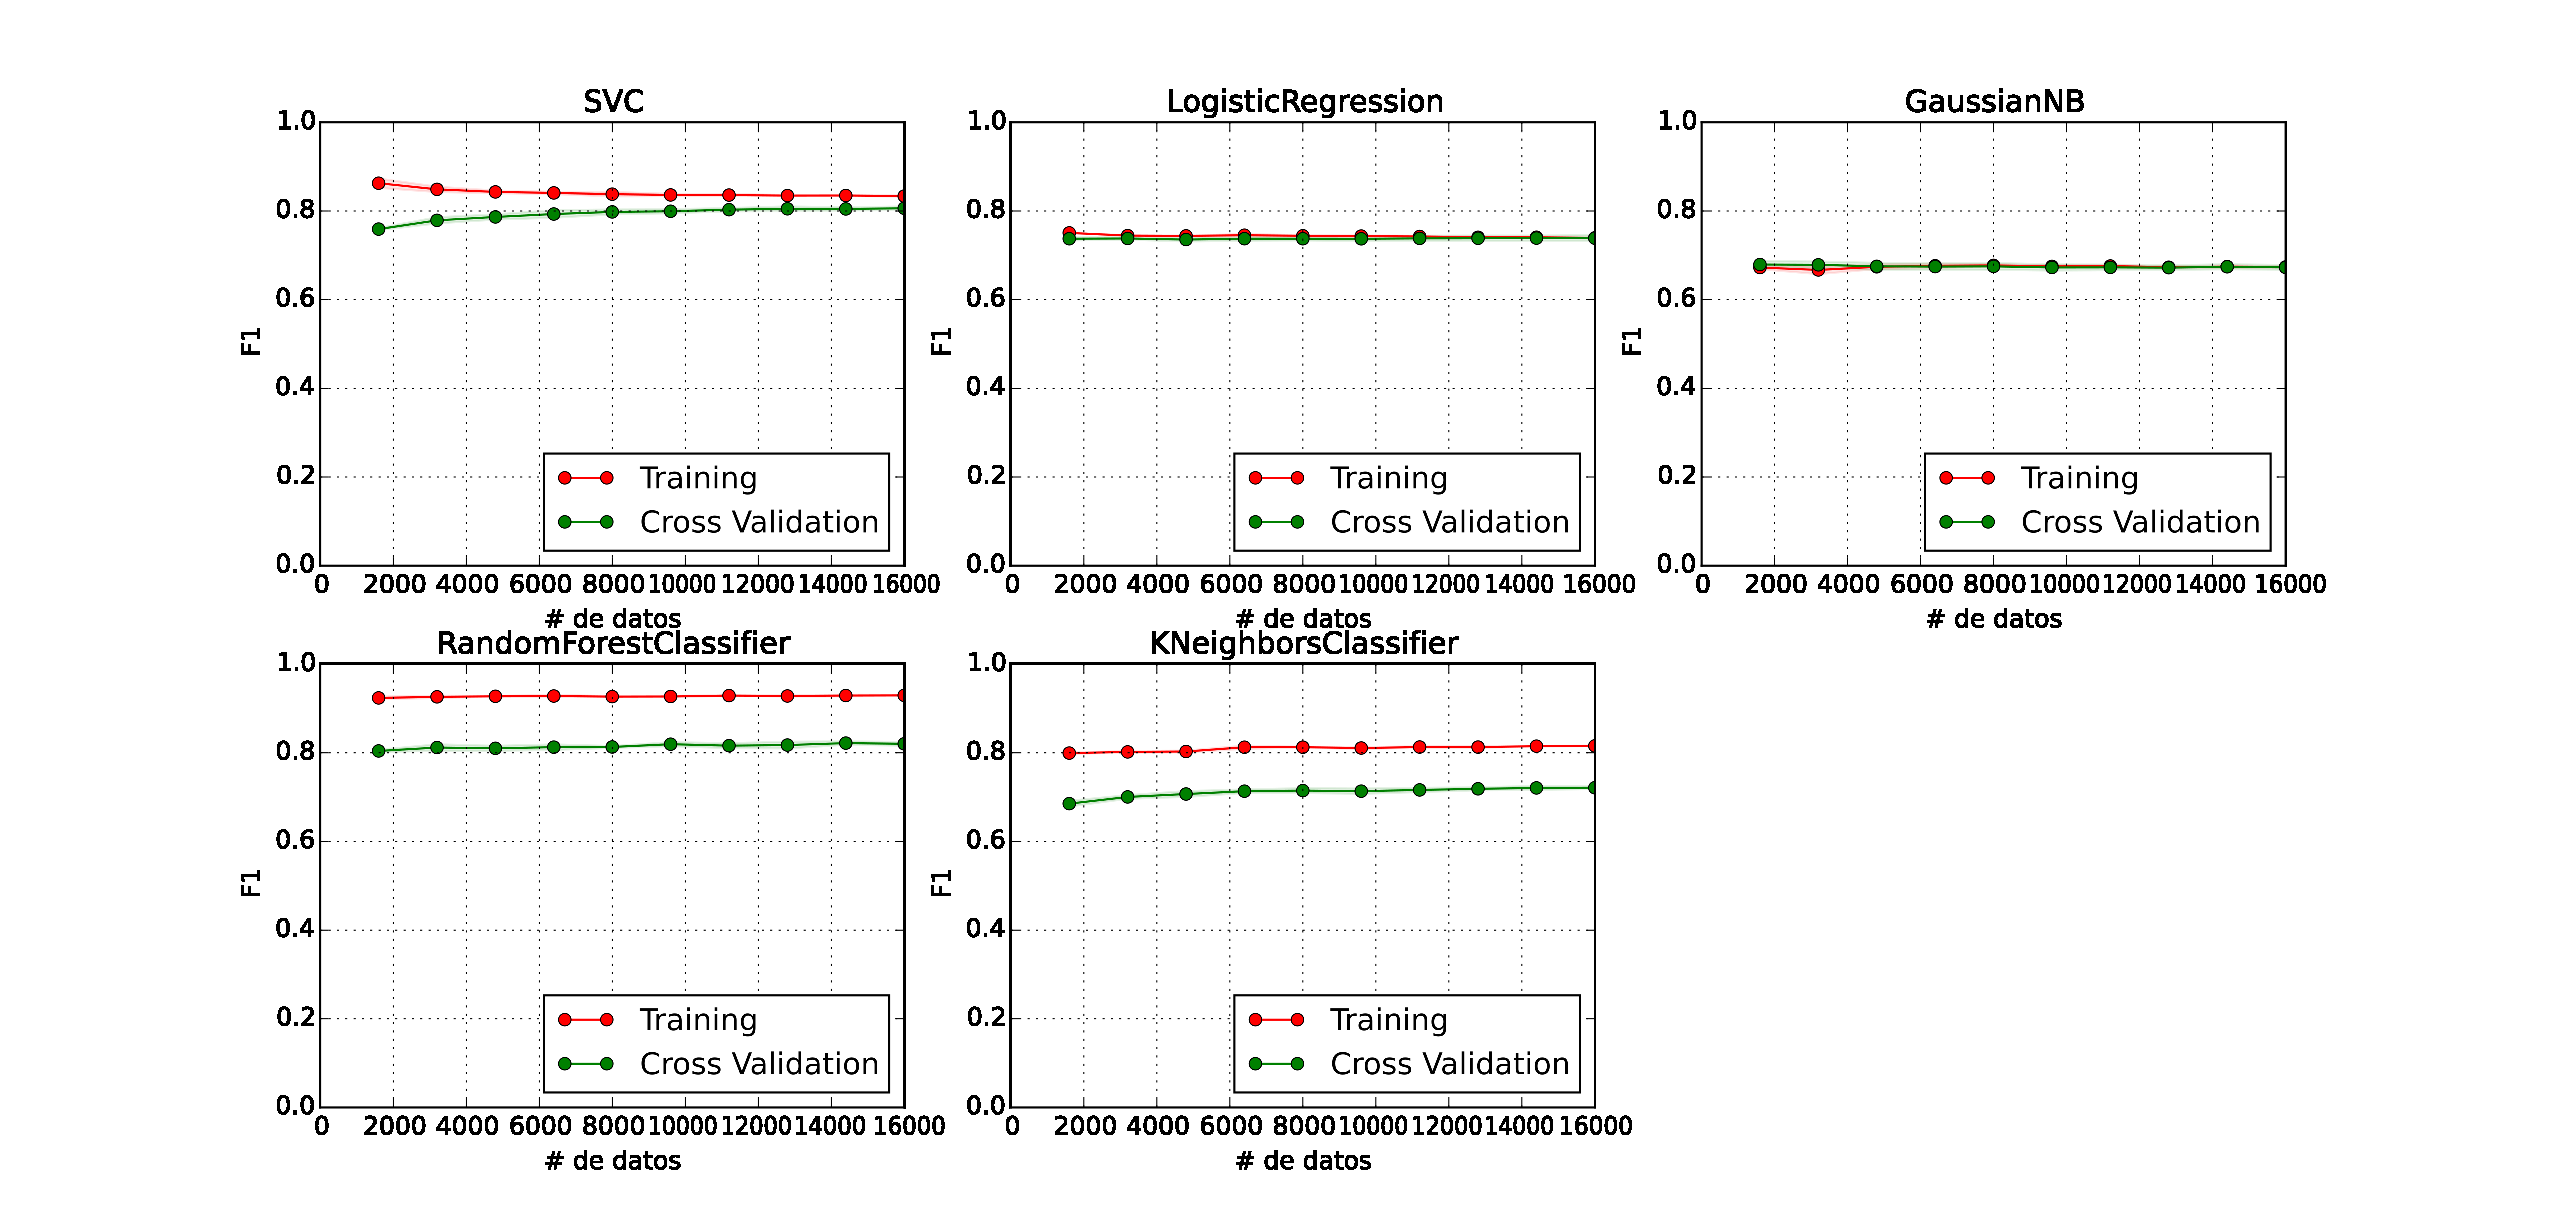
\includegraphics[width=1.00\textwidth]{higgs,_curvas_de_aprendizaje_post_CV}
	\end{figure}
\end{frame}
	

\begin{frame}
	\frametitle{Resultados}
	El c\'odigo utilizado para los c\'alculos de este trabajo ha sido realizado en Python, con ayuda del paquete de Inteligencia Artificial \texttt{scikit-learn}. 

	Todos los c\'alculos han sido llevados a cabo por un ordenador con sistema operativo Windows 7 de 64 bits, un procesador Intel$^\circledR$ Core\texttrademark \ i3 a 1.7 GHz, con 4 GB de memoria RAM.

Todo el c\'odigo, datos y gr\'aficas vienen recogidos en el CD con material suplementario entregado junto a la memoria del trabajo.
\end{frame}

\end{document}
